\chapter{Autoencoders}

Now, having introduced the basics of neural networks in Chapter \ref{preliminary} we can consider a specific architecture of a neural network, a so called autoencoder neural network, or short: autoencoders. The conceptional idea of autoencoders is to take a given input, compress (usually called encore) the input to a given size and afterwards, expand (usually called decode) it as close as possible to the original representation again. Such an architecture is widely used in different areas. For example on social media platforms - where users send images to one another. Instead of sending the original image, which size might very well be a couple of megabytes, the image is being encoded first and sent in the compressed representation. Afterwards, the recipient decodes the image to its original representation. This way one has only to transmit the encoded representation, which usually is smaller by magnitudes.
Another very important application of autoencoders is in the Machine Learning field. Most state of the art Machine Learning models are using autoencoders, since it is way more efficient to first encode the data and then fit the model on the encoded data. This is quite straight-forward, considering the same argument as in the previous use-case - the encoded data being smaller by magnitudes. This way firstly, processing the samples can happen much faster compared to the non-encoded data samples and secondly, it makes storing data (on the drive and in memory) much more efficient.\\
The conceptional idea of autoencoders is now clear, but how exactly would one formulate such an architecture mathematically? This is the central question we want to answer in this chapter.

\section{Mathematical formulation of autoencoders}

As already mentioned, the input data is firstly being encoded, and afterwards it is being decoded. Hence, we can divide these two steps into separate architectures - the encoder and the decoder, which we will formulate separately. In figure \ref{autoencoder} we can take a look at a visual example of an autoencoder architecture.


\begin{figure}[H]
\begin{center}
   \begin{minipage}[b]{0.9\linewidth}
      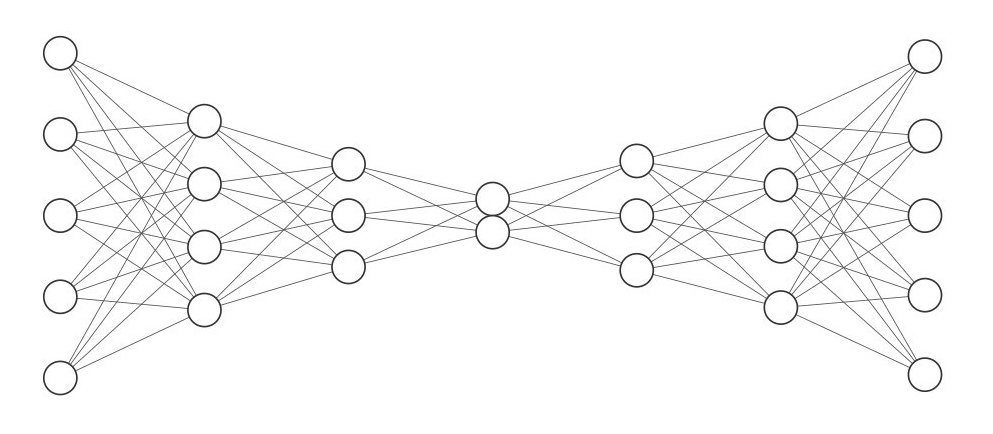
\includegraphics[width=\linewidth]{autoencoder}
      \caption{An autoencoder neural network with input and output $x, y\in \R^5$. The five hidden layers have dimensions $4$, $3$, $2$, $3$ and $4$ respectively. Hence, the bottleneck dimension is $2$ in this example. The graphic was generated with http://alexlenail.me/NN-SVG/index.html}\label{autoencoder}
	\end{minipage}
\end{center}
\end{figure}


If we divide the autoencoder as described above, we firstly obtain the encoder as we can see in figure \ref{img_encoder}. Or formally defined as follows

\begin{lemma}\label{def_encoder}
Let $\T$ be a parameter space and $\t \in \T$ a parameter, $L\in \N$ and $d_1,\ldots, d_L\in\N$. Let further $\f$ be an activation function and $f_{\f,L,\t}$ a neural network.\\
If the neural network $f_{\f,L,\t}$ fulfils the condition $n_i= d_1 \geq \ldots, \geq d_L = n_o$ with $n_i, n_o \in \N$ being the input and output dimensions respectively, then we speak of an \textbf{encoding neural network} (or short: \textbf{encoder}).
\end{lemma}


\begin{figure}[H]
\begin{center}
   \begin{minipage}[b]{0.9\linewidth}
      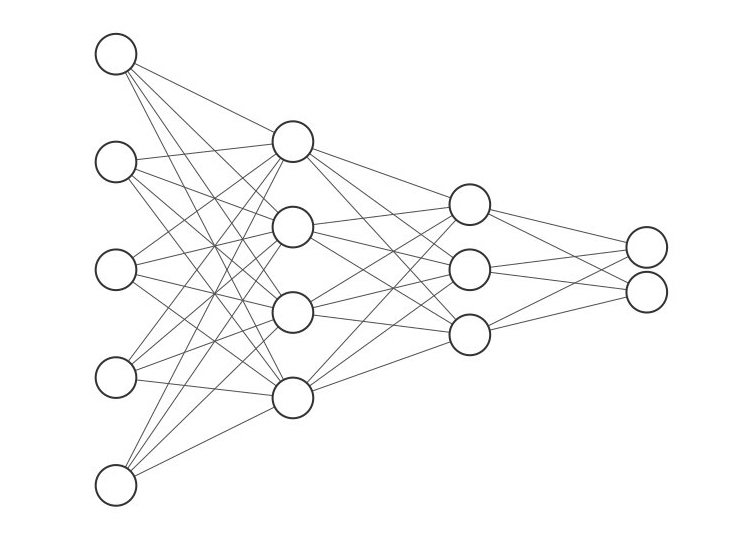
\includegraphics[width=\linewidth]{encoder}
      \caption{An encoder neural network with input $x\in \R^5$ and output $y \in \R^2$. The two hidden layers have dimensions $4$ and $3$. Hence, the encoder reduces the data dimensionality from $5$ to $2$ dimension. The graphic was generated with http://alexlenail.me/NN-SVG/index.html}\label{img_encoder}
	\end{minipage}
\end{center}
\end{figure}


For the second part of the divided autoencoder structure, we obtain the decoder as we can see in figure \ref{img_decoder}. We can define this architecture analogously to the encoder in lemma \ref{def_encoder}.


\begin{lemma}\label{def_decoder}
Let $\T$ be a parameter space and $\t \in \T$ a parameter, $L\in \N$ and $d_1,\ldots, d_L\in\N$. Let further $\f$ be an activation function and $f_{\f,L,\t}$ a neural network.\\
If the neural network $f_{\f,L,\t}$ fulfils the condition $n_i= d_1 \leq \ldots, \leq d_L = n_o$ with $n_i, n_o \in \N$ being the input and output dimensions respectively, then we speak of an \textbf{decoding neural network} (or short: \textbf{decoder}).
\end{lemma}


\begin{figure}[H]
\begin{center}
   \begin{minipage}[b]{0.9\linewidth}
      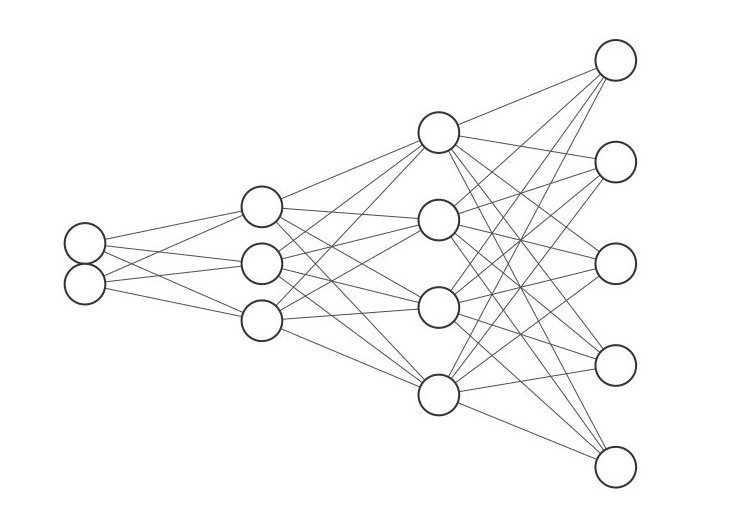
\includegraphics[width=\linewidth]{decoder}
      \caption{A decoder neural network with input $x\in \R^2$ and output $y \in \R^5$. The two hidden layers have dimensions $3$ and $4$. Hence, the decoder expands the data dimensionality from $2$ to $5$ dimensions. The graphic was generated with http://alexlenail.me/NN-SVG/index.html}\label{img_decoder}
	\end{minipage}
\end{center}
\end{figure}
